\hypertarget{sample2_8c}{
\section{sample2.c File Reference}
\label{sample2_8c}\index{sample2.c@{sample2.c}}
}
{\tt \#include $<$linux/module.h$>$}\par
{\tt \#include $<$linux/kernel.h$>$}\par
{\tt \#include $<$linux/init.h$>$}\par
{\tt \#include $<$linux/fs.h$>$}\par
{\tt \#include $<$asm/uaccess.h$>$}\par


Include dependency graph for sample2.c:\begin{figure}[H]
\begin{center}
\leavevmode
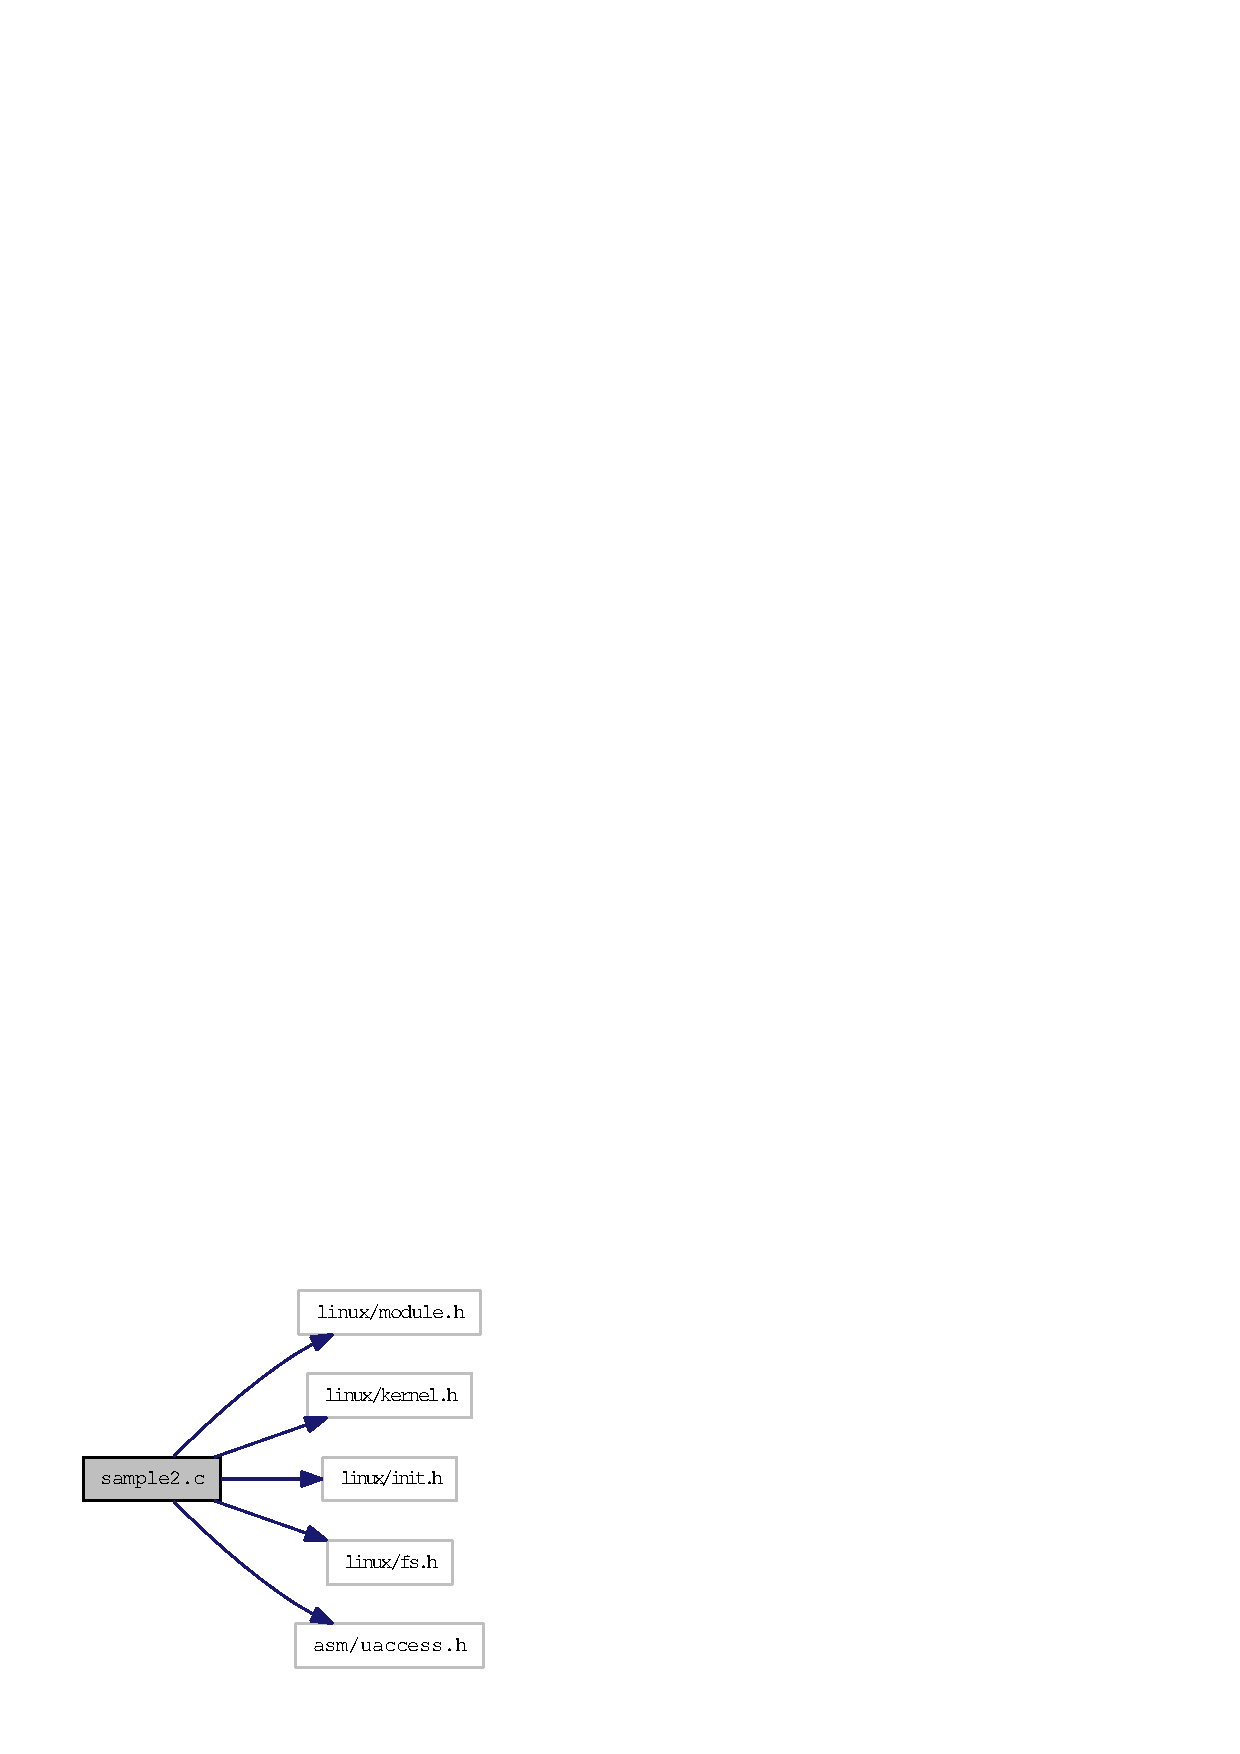
\includegraphics[width=118pt]{sample2_8c__incl}
\end{center}
\end{figure}
\subsection*{Defines}
\begin{CompactItemize}
\item 
\#define \hyperlink{sample2_8c_a65afd64a86d56e9b4fcf7c6aa51ad0b}{d\_\-printk}(level, fmt, args...)
\end{CompactItemize}
\subsection*{Functions}
\begin{CompactItemize}
\item 
\hyperlink{sample2_8c_ef39319fa1de091a1f8e72c928856c1c}{module\_\-param} (\hyperlink{sample2_8c_d6a45be35a0fd6945a28335390ccba44}{sample\_\-debug}, int, S\_\-IRUSR$|$S\_\-IWUSR)
\item 
\hyperlink{sample2_8c_18d24c1000ff14aef0b1b67a60762ee5}{MODULE\_\-PARM\_\-DESC} (\hyperlink{sample2_8c_d6a45be35a0fd6945a28335390ccba44}{sample\_\-debug},\char`\"{}Sample driver verbosity level\char`\"{})
\item 
\hyperlink{sample2_8c_926962b8a541fe2e09225c14b36df624}{module\_\-param} (\hyperlink{sample2_8c_006e34b70c4b79c4dfec8cacf1abbfde}{sample\_\-major}, uint, S\_\-IRUSR$|$S\_\-IWUSR)
\item 
\hyperlink{sample2_8c_940ee54b59f3a44c15064925e230e725}{MODULE\_\-PARM\_\-DESC} (\hyperlink{sample2_8c_006e34b70c4b79c4dfec8cacf1abbfde}{sample\_\-major},\char`\"{}Sample driver major number\char`\"{})
\item 
static int \hyperlink{sample2_8c_7a632696036498f99c4a9afcaae60d90}{sample\_\-open} (struct inode $\ast$inode, struct file $\ast$file)
\item 
static int \hyperlink{sample2_8c_92618d8e7f647c43e5a53ff4f2f242ea}{sample\_\-release} (struct inode $\ast$inode, struct file $\ast$file)
\item 
static ssize\_\-t \hyperlink{sample2_8c_3d9e454fcca8444eb0485f84c9d932ef}{sample\_\-read} (struct file $\ast$filp, char $\ast$buffer, size\_\-t length, loff\_\-t $\ast$offset)
\item 
static ssize\_\-t \hyperlink{sample2_8c_d112fcdb00825baaf14f39bc8dce2854}{sample\_\-write} (struct file $\ast$filp, const char $\ast$buffer, size\_\-t length, loff\_\-t $\ast$offset)
\item 
static int \_\-\_\-init \hyperlink{sample2_8c_24e096d93827eff8ab8f6ee6bf636bf3}{sample\_\-init\_\-module} (void)
\item 
static void \_\-\_\-exit \hyperlink{sample2_8c_57811ec32fa4897a3d57e92b5fd73c16}{sample\_\-cleanup\_\-module} (void)
\item 
\hyperlink{sample2_8c_dc12b685b9b55f3050ddf618513de15c}{module\_\-init} (sample\_\-init\_\-module)
\item 
\hyperlink{sample2_8c_338956505e745aa0d89744419df172e3}{module\_\-exit} (sample\_\-cleanup\_\-module)
\item 
\hyperlink{sample2_8c_d94b36675e7eb067ea3ce6ff9e244a44}{MODULE\_\-LICENSE} (\char`\"{}GPL\char`\"{})
\item 
\hyperlink{sample2_8c_39c932e75726f9dacdfc03e622fae810}{MODULE\_\-AUTHOR} (\char`\"{}Vladimir Khusainov, vlad@emcraft.com\char`\"{})
\item 
\hyperlink{sample2_8c_e6cd2f58493cacec7a8dc2ad4c6cc888}{MODULE\_\-DESCRIPTION} (\char`\"{}Sample device driver\char`\"{})
\end{CompactItemize}
\subsection*{Variables}
\begin{CompactItemize}
\item 
static int \hyperlink{sample2_8c_d6a45be35a0fd6945a28335390ccba44}{sample\_\-debug} = 0
\item 
static uint \hyperlink{sample2_8c_006e34b70c4b79c4dfec8cacf1abbfde}{sample\_\-major} = 166
\item 
static char $\ast$ \hyperlink{sample2_8c_73d6ad39f8437a25e890ca32bcbaa29c}{sample\_\-name} = \char`\"{}sample\char`\"{}
\item 
static int \hyperlink{sample2_8c_a97ad4291bd64d39b97f0fcc30856cb5}{sample\_\-lock} = 0
\item 
static char \hyperlink{sample2_8c_508e3a03408c5f0d53480650ecae7c61}{sample\_\-str} \mbox{[}$\,$\mbox{]} = \char`\"{}This is the simplest loadable kernel module!!!! sample.ko$\backslash$n\char`\"{}
\item 
static char $\ast$ \hyperlink{sample2_8c_4480e78f1a47158fd65d2c8c938aca0e}{sample\_\-end}
\item 
static struct file\_\-operations \hyperlink{sample2_8c_9e76433fdf0e65c77ed48c656b0444ca}{sample\_\-fops}
\end{CompactItemize}


\subsection{Define Documentation}
\hypertarget{sample2_8c_a65afd64a86d56e9b4fcf7c6aa51ad0b}{
\index{sample2.c@{sample2.c}!d_printk@{d\_\-printk}}
\index{d_printk@{d\_\-printk}!sample2.c@{sample2.c}}
\subsubsection[d\_\-printk]{\setlength{\rightskip}{0pt plus 5cm}\#define d\_\-printk(level, fmt, args...)}}
\label{sample2_8c_a65afd64a86d56e9b4fcf7c6aa51ad0b}


\textbf{Value:}

\begin{Code}\begin{verbatim}if (sample_debug >= level) printk(KERN_INFO "%s: " fmt, \
                    __func__, ## args)
\end{verbatim}\end{Code}


Definition at line 27 of file sample2.c.

\subsection{Function Documentation}
\hypertarget{sample2_8c_39c932e75726f9dacdfc03e622fae810}{
\index{sample2.c@{sample2.c}!MODULE_AUTHOR@{MODULE\_\-AUTHOR}}
\index{MODULE_AUTHOR@{MODULE\_\-AUTHOR}!sample2.c@{sample2.c}}
\subsubsection[MODULE\_\-AUTHOR]{\setlength{\rightskip}{0pt plus 5cm}MODULE\_\-AUTHOR (\char`\"{}Vladimir  {\em Khusainov}, vlad @emcraft.com\char`\"{})}}
\label{sample2_8c_39c932e75726f9dacdfc03e622fae810}


\hypertarget{sample2_8c_e6cd2f58493cacec7a8dc2ad4c6cc888}{
\index{sample2.c@{sample2.c}!MODULE_DESCRIPTION@{MODULE\_\-DESCRIPTION}}
\index{MODULE_DESCRIPTION@{MODULE\_\-DESCRIPTION}!sample2.c@{sample2.c}}
\subsubsection[MODULE\_\-DESCRIPTION]{\setlength{\rightskip}{0pt plus 5cm}MODULE\_\-DESCRIPTION (\char`\"{}Sample device driver\char`\"{})}}
\label{sample2_8c_e6cd2f58493cacec7a8dc2ad4c6cc888}


\hypertarget{sample2_8c_338956505e745aa0d89744419df172e3}{
\index{sample2.c@{sample2.c}!module_exit@{module\_\-exit}}
\index{module_exit@{module\_\-exit}!sample2.c@{sample2.c}}
\subsubsection[module\_\-exit]{\setlength{\rightskip}{0pt plus 5cm}module\_\-exit (sample\_\-cleanup\_\-module)}}
\label{sample2_8c_338956505e745aa0d89744419df172e3}


\hypertarget{sample2_8c_dc12b685b9b55f3050ddf618513de15c}{
\index{sample2.c@{sample2.c}!module_init@{module\_\-init}}
\index{module_init@{module\_\-init}!sample2.c@{sample2.c}}
\subsubsection[module\_\-init]{\setlength{\rightskip}{0pt plus 5cm}module\_\-init (sample\_\-init\_\-module)}}
\label{sample2_8c_dc12b685b9b55f3050ddf618513de15c}


\hypertarget{sample2_8c_d94b36675e7eb067ea3ce6ff9e244a44}{
\index{sample2.c@{sample2.c}!MODULE_LICENSE@{MODULE\_\-LICENSE}}
\index{MODULE_LICENSE@{MODULE\_\-LICENSE}!sample2.c@{sample2.c}}
\subsubsection[MODULE\_\-LICENSE]{\setlength{\rightskip}{0pt plus 5cm}MODULE\_\-LICENSE (\char`\"{}GPL\char`\"{})}}
\label{sample2_8c_d94b36675e7eb067ea3ce6ff9e244a44}


\hypertarget{sample2_8c_926962b8a541fe2e09225c14b36df624}{
\index{sample2.c@{sample2.c}!module_param@{module\_\-param}}
\index{module_param@{module\_\-param}!sample2.c@{sample2.c}}
\subsubsection[module\_\-param]{\setlength{\rightskip}{0pt plus 5cm}module\_\-param (\hyperlink{sample2_8c_006e34b70c4b79c4dfec8cacf1abbfde}{sample\_\-major}, uint, S\_\-IRUSR$|$ {\em S\_\-IWUSR})}}
\label{sample2_8c_926962b8a541fe2e09225c14b36df624}


\hypertarget{sample2_8c_ef39319fa1de091a1f8e72c928856c1c}{
\index{sample2.c@{sample2.c}!module_param@{module\_\-param}}
\index{module_param@{module\_\-param}!sample2.c@{sample2.c}}
\subsubsection[module\_\-param]{\setlength{\rightskip}{0pt plus 5cm}module\_\-param (\hyperlink{sample2_8c_d6a45be35a0fd6945a28335390ccba44}{sample\_\-debug}, int, S\_\-IRUSR$|$ {\em S\_\-IWUSR})}}
\label{sample2_8c_ef39319fa1de091a1f8e72c928856c1c}


\hypertarget{sample2_8c_940ee54b59f3a44c15064925e230e725}{
\index{sample2.c@{sample2.c}!MODULE_PARM_DESC@{MODULE\_\-PARM\_\-DESC}}
\index{MODULE_PARM_DESC@{MODULE\_\-PARM\_\-DESC}!sample2.c@{sample2.c}}
\subsubsection[MODULE\_\-PARM\_\-DESC]{\setlength{\rightskip}{0pt plus 5cm}MODULE\_\-PARM\_\-DESC (\hyperlink{sample2_8c_006e34b70c4b79c4dfec8cacf1abbfde}{sample\_\-major}, \char`\"{}Sample driver major number\char`\"{})}}
\label{sample2_8c_940ee54b59f3a44c15064925e230e725}


\hypertarget{sample2_8c_18d24c1000ff14aef0b1b67a60762ee5}{
\index{sample2.c@{sample2.c}!MODULE_PARM_DESC@{MODULE\_\-PARM\_\-DESC}}
\index{MODULE_PARM_DESC@{MODULE\_\-PARM\_\-DESC}!sample2.c@{sample2.c}}
\subsubsection[MODULE\_\-PARM\_\-DESC]{\setlength{\rightskip}{0pt plus 5cm}MODULE\_\-PARM\_\-DESC (\hyperlink{sample2_8c_d6a45be35a0fd6945a28335390ccba44}{sample\_\-debug}, \char`\"{}Sample driver verbosity level\char`\"{})}}
\label{sample2_8c_18d24c1000ff14aef0b1b67a60762ee5}


\hypertarget{sample2_8c_57811ec32fa4897a3d57e92b5fd73c16}{
\index{sample2.c@{sample2.c}!sample_cleanup_module@{sample\_\-cleanup\_\-module}}
\index{sample_cleanup_module@{sample\_\-cleanup\_\-module}!sample2.c@{sample2.c}}
\subsubsection[sample\_\-cleanup\_\-module]{\setlength{\rightskip}{0pt plus 5cm}static void \_\-\_\-exit sample\_\-cleanup\_\-module (void)\hspace{0.3cm}{\tt  \mbox{[}static\mbox{]}}}}
\label{sample2_8c_57811ec32fa4897a3d57e92b5fd73c16}




Definition at line 202 of file sample2.c.

References d\_\-printk, sample\_\-major, and sample\_\-name.\hypertarget{sample2_8c_24e096d93827eff8ab8f6ee6bf636bf3}{
\index{sample2.c@{sample2.c}!sample_init_module@{sample\_\-init\_\-module}}
\index{sample_init_module@{sample\_\-init\_\-module}!sample2.c@{sample2.c}}
\subsubsection[sample\_\-init\_\-module]{\setlength{\rightskip}{0pt plus 5cm}static int \_\-\_\-init sample\_\-init\_\-module (void)\hspace{0.3cm}{\tt  \mbox{[}static\mbox{]}}}}
\label{sample2_8c_24e096d93827eff8ab8f6ee6bf636bf3}




Definition at line 173 of file sample2.c.

References d\_\-printk, sample\_\-fops, sample\_\-major, and sample\_\-name.\hypertarget{sample2_8c_7a632696036498f99c4a9afcaae60d90}{
\index{sample2.c@{sample2.c}!sample_open@{sample\_\-open}}
\index{sample_open@{sample\_\-open}!sample2.c@{sample2.c}}
\subsubsection[sample\_\-open]{\setlength{\rightskip}{0pt plus 5cm}static int sample\_\-open (struct inode $\ast$ {\em inode}, struct file $\ast$ {\em file})\hspace{0.3cm}{\tt  \mbox{[}static\mbox{]}}}}
\label{sample2_8c_7a632696036498f99c4a9afcaae60d90}




Definition at line 62 of file sample2.c.

References d\_\-printk, sample\_\-end, sample\_\-lock, and sample\_\-str.\hypertarget{sample2_8c_3d9e454fcca8444eb0485f84c9d932ef}{
\index{sample2.c@{sample2.c}!sample_read@{sample\_\-read}}
\index{sample_read@{sample\_\-read}!sample2.c@{sample2.c}}
\subsubsection[sample\_\-read]{\setlength{\rightskip}{0pt plus 5cm}static ssize\_\-t sample\_\-read (struct file $\ast$ {\em filp}, char $\ast$ {\em buffer}, size\_\-t {\em length}, loff\_\-t $\ast$ {\em offset})\hspace{0.3cm}{\tt  \mbox{[}static\mbox{]}}}}
\label{sample2_8c_3d9e454fcca8444eb0485f84c9d932ef}




Definition at line 111 of file sample2.c.

References d\_\-printk, sample\_\-end, and sample\_\-str.\hypertarget{sample2_8c_92618d8e7f647c43e5a53ff4f2f242ea}{
\index{sample2.c@{sample2.c}!sample_release@{sample\_\-release}}
\index{sample_release@{sample\_\-release}!sample2.c@{sample2.c}}
\subsubsection[sample\_\-release]{\setlength{\rightskip}{0pt plus 5cm}static int sample\_\-release (struct inode $\ast$ {\em inode}, struct file $\ast$ {\em file})\hspace{0.3cm}{\tt  \mbox{[}static\mbox{]}}}}
\label{sample2_8c_92618d8e7f647c43e5a53ff4f2f242ea}




Definition at line 92 of file sample2.c.

References d\_\-printk, and sample\_\-lock.\hypertarget{sample2_8c_d112fcdb00825baaf14f39bc8dce2854}{
\index{sample2.c@{sample2.c}!sample_write@{sample\_\-write}}
\index{sample_write@{sample\_\-write}!sample2.c@{sample2.c}}
\subsubsection[sample\_\-write]{\setlength{\rightskip}{0pt plus 5cm}static ssize\_\-t sample\_\-write (struct file $\ast$ {\em filp}, const char $\ast$ {\em buffer}, size\_\-t {\em length}, loff\_\-t $\ast$ {\em offset})\hspace{0.3cm}{\tt  \mbox{[}static\mbox{]}}}}
\label{sample2_8c_d112fcdb00825baaf14f39bc8dce2854}




Definition at line 156 of file sample2.c.

References d\_\-printk.

\subsection{Variable Documentation}
\hypertarget{sample2_8c_d6a45be35a0fd6945a28335390ccba44}{
\index{sample2.c@{sample2.c}!sample_debug@{sample\_\-debug}}
\index{sample_debug@{sample\_\-debug}!sample2.c@{sample2.c}}
\subsubsection[sample\_\-debug]{\setlength{\rightskip}{0pt plus 5cm}int \hyperlink{sample2_8c_d6a45be35a0fd6945a28335390ccba44}{sample\_\-debug} = 0\hspace{0.3cm}{\tt  \mbox{[}static\mbox{]}}}}
\label{sample2_8c_d6a45be35a0fd6945a28335390ccba44}




Definition at line 16 of file sample2.c.\hypertarget{sample2_8c_4480e78f1a47158fd65d2c8c938aca0e}{
\index{sample2.c@{sample2.c}!sample_end@{sample\_\-end}}
\index{sample_end@{sample\_\-end}!sample2.c@{sample2.c}}
\subsubsection[sample\_\-end]{\setlength{\rightskip}{0pt plus 5cm}char$\ast$ \hyperlink{sample2_8c_4480e78f1a47158fd65d2c8c938aca0e}{sample\_\-end}\hspace{0.3cm}{\tt  \mbox{[}static\mbox{]}}}}
\label{sample2_8c_4480e78f1a47158fd65d2c8c938aca0e}




Definition at line 57 of file sample2.c.\hypertarget{sample2_8c_9e76433fdf0e65c77ed48c656b0444ca}{
\index{sample2.c@{sample2.c}!sample_fops@{sample\_\-fops}}
\index{sample_fops@{sample\_\-fops}!sample2.c@{sample2.c}}
\subsubsection[sample\_\-fops]{\setlength{\rightskip}{0pt plus 5cm}struct file\_\-operations \hyperlink{sample2_8c_9e76433fdf0e65c77ed48c656b0444ca}{sample\_\-fops}\hspace{0.3cm}{\tt  \mbox{[}static\mbox{]}}}}
\label{sample2_8c_9e76433fdf0e65c77ed48c656b0444ca}


\textbf{Initial value:}

\begin{Code}\begin{verbatim} {
  .read = sample_read,
  .write = sample_write,
  .open = sample_open,
  .release = sample_release
}
\end{verbatim}\end{Code}


Definition at line 166 of file sample2.c.\hypertarget{sample2_8c_a97ad4291bd64d39b97f0fcc30856cb5}{
\index{sample2.c@{sample2.c}!sample_lock@{sample\_\-lock}}
\index{sample_lock@{sample\_\-lock}!sample2.c@{sample2.c}}
\subsubsection[sample\_\-lock]{\setlength{\rightskip}{0pt plus 5cm}int \hyperlink{sample2_8c_a97ad4291bd64d39b97f0fcc30856cb5}{sample\_\-lock} = 0\hspace{0.3cm}{\tt  \mbox{[}static\mbox{]}}}}
\label{sample2_8c_a97ad4291bd64d39b97f0fcc30856cb5}




Definition at line 51 of file sample2.c.\hypertarget{sample2_8c_006e34b70c4b79c4dfec8cacf1abbfde}{
\index{sample2.c@{sample2.c}!sample_major@{sample\_\-major}}
\index{sample_major@{sample\_\-major}!sample2.c@{sample2.c}}
\subsubsection[sample\_\-major]{\setlength{\rightskip}{0pt plus 5cm}uint \hyperlink{sample2_8c_006e34b70c4b79c4dfec8cacf1abbfde}{sample\_\-major} = 166\hspace{0.3cm}{\tt  \mbox{[}static\mbox{]}}}}
\label{sample2_8c_006e34b70c4b79c4dfec8cacf1abbfde}




Definition at line 34 of file sample2.c.\hypertarget{sample2_8c_73d6ad39f8437a25e890ca32bcbaa29c}{
\index{sample2.c@{sample2.c}!sample_name@{sample\_\-name}}
\index{sample_name@{sample\_\-name}!sample2.c@{sample2.c}}
\subsubsection[sample\_\-name]{\setlength{\rightskip}{0pt plus 5cm}char$\ast$ \hyperlink{sample2_8c_73d6ad39f8437a25e890ca32bcbaa29c}{sample\_\-name} = \char`\"{}sample\char`\"{}\hspace{0.3cm}{\tt  \mbox{[}static\mbox{]}}}}
\label{sample2_8c_73d6ad39f8437a25e890ca32bcbaa29c}




Definition at line 45 of file sample2.c.\hypertarget{sample2_8c_508e3a03408c5f0d53480650ecae7c61}{
\index{sample2.c@{sample2.c}!sample_str@{sample\_\-str}}
\index{sample_str@{sample\_\-str}!sample2.c@{sample2.c}}
\subsubsection[sample\_\-str]{\setlength{\rightskip}{0pt plus 5cm}char \hyperlink{sample2_8c_508e3a03408c5f0d53480650ecae7c61}{sample\_\-str}\mbox{[}$\,$\mbox{]} = \char`\"{}This is the simplest loadable kernel module!!!! sample.ko$\backslash$n\char`\"{}\hspace{0.3cm}{\tt  \mbox{[}static\mbox{]}}}}
\label{sample2_8c_508e3a03408c5f0d53480650ecae7c61}




Definition at line 56 of file sample2.c.